\chapter{Implementation}

\section{DEAP Framework}

\par
The chosen framework for the implementation is DEAP \cite{DEAP_JMLR2012}.
DEAP (Distributed Evolutionary Algorithms in Python) is a Python library that excels at rapid prototyping and testing of ideas, making the tool ideal for the project.

\section{Gene Representation}

The gene representation is a binary string, where each bit represents the presence of a vertex in the solution.
The length of the string is equal to the number of vertices in the graph.
The weight of the vertex is stored in a separate list, where the index corresponds to the vertex index.

\begin{figure}[ht]
\centering
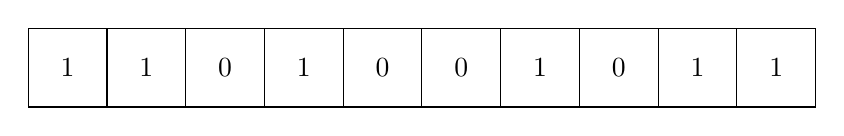
\begin{tikzpicture}
	\foreach \i in {1,2,4,7,9,10} {
		\draw (\i,0) rectangle (\i+1,1);
		\node at (\i+0.5,0.5) {1};
		}
	\foreach \i in {3,5,6,8} {
		\draw (\i,0) rectangle (\i+1,1);
		\node at (\i+0.5,0.5) {0};
	}
\end{tikzpicture}
\caption{Example of a MWVC gene representation}
\end{figure}

\section{Fitness Function}

The fitness function for the Minimum Weight Vertex Cover problem calculates the weight of the solution by summing the weights of the vertices present in the solution.
Additionally, it imposes a penalty for each edge that is not covered by the vertices in the solution, ensuring that the fitness value is higher for incomplete solutions.
The penalty function (or a similar alternative) is mandatory since we're using a direct gene representation that could create invalid configurations of uncovered vertices.

\begin{framed}
\begin{lstlisting}[caption=Fitness function]
function fitness(individual)
	f = 0
	for i in 0..n-1
		if individual[i] == 1
			f = f + vertex_weight[i]
		end
	end

	for edge in graph.edges
		if individual[edge.from] == 0 and individual[edge.to] == 0
			f = f + penalty
		end
	end
	return f
end
\end{lstlisting}
\end{framed}

The objective function is the same but with a penalty of zero, and it returns $\text{NULL}$ if the solution is invalid (i.e. there are uncovered edges).



\section{Performance Metrics}

In order to evaluate the performance of the algorithm, it is necessary to define a set of metrics to evaluate the quality of the solution and the performance of the algorithm.

The most important one is the fitness, as well as the objective (that does not include the penalties). Another metric to optimize is the number of evaluations, as it is a direct measure of the computational cost of the algorithm.

The execution time is not considered as a metric as it is highly dependent on the hardware and software environment.

It would be useful to include an optimality metric representing the difference between the best known solution and the solution found by the algorithm, but this information is not easily computable as the problem is NP-hard.

\section{Parameters}

Genetic Algorithms have a set of parameters that need to be tuned in order to achieve the best performance.

The following is the list of the meta-parameters configurable in the implementation:

\begin{itemize}
	\item \textbf{Population size} (\texttt{POPULATION\_SIZE}): the number of individuals in the population.
	\item \textbf{Crossover probability} (\texttt{CXPB}): the probability of crossover.
	\item \textbf{Mutation probability} (\texttt{MUTPB}): the probability of mutation.
	\item \textbf{k-tournament selection size} (\texttt{K\_TOURNAMENT}): the size $k$ of the tournament in the k-tournament selection.
	\item \textbf{Number of generations} (\texttt{NUMBER\_OF\_GENERATIONS}): the number of generations the algorithm will run.
\end{itemize}

The problem of finding the best parameters is an optimization problem itself, and it is possible to use a meta-heuristic algorithm to find the best parameters, such as a Genetic Algorithm \cite{meta-heuristic}. This is out of the scope of this project even though it could be an interesting future development.

\section{Benchmarking Flow}

This paragraph describes the flow of the benchmarking process. The goal of the benchmarking process is to test the algorithm with a fixed parameters combination over different graph instances to extract the metrics and evaluate the performance of the algorithm. The parameters are chosen based on the literature and are discussed in the chapter 4.

The process is divided into the following steps:

\begin{enumerate}
	\item \textbf{Load the graphs}: the problem instances for testing are loaded from the files.
	\item \textbf{Compute graphs properties}: for each graph a set of properties are computed, such as the number of vertices, the number of edges and the density.
	\item \textbf{Create the DEAP structures}: the DEAP structures are created, including the individuals, the population and the evaluation function.
	\item \textbf{Run the algorithm}: the algorithm is executed with the set parameters over the graph instances.
	\item \textbf{Save the results}: the results are saved to a multiple files in JSON format for further analysis.
	\item \textbf{Analyze the results}: the results are analyzed to extract the metrics and evaluate the performance of the algorithm.
\end{enumerate}

Every step, except the last one, is executed within a Python script with configurable parameters. The last step is performed using a Jupyter Notebook for a faster and more interactive analysis.

The benchmarking process is repeated iteratively over different parameters combinations to find the best configuration for the algorithm.

